\PassOptionsToPackage{unicode=true}{hyperref} % options for packages loaded elsewhere
\PassOptionsToPackage{hyphens}{url}
%
\documentclass[]{article}
\usepackage{lmodern}
\usepackage{amssymb,amsmath}
\usepackage{ifxetex,ifluatex}
\usepackage{fixltx2e} % provides \textsubscript
\ifnum 0\ifxetex 1\fi\ifluatex 1\fi=0 % if pdftex
  \usepackage[T1]{fontenc}
  \usepackage[utf8]{inputenc}
  \usepackage{textcomp} % provides euro and other symbols
\else % if luatex or xelatex
  \usepackage{unicode-math}
  \defaultfontfeatures{Ligatures=TeX,Scale=MatchLowercase}
\fi
% use upquote if available, for straight quotes in verbatim environments
\IfFileExists{upquote.sty}{\usepackage{upquote}}{}
% use microtype if available
\IfFileExists{microtype.sty}{%
\usepackage[]{microtype}
\UseMicrotypeSet[protrusion]{basicmath} % disable protrusion for tt fonts
}{}
\IfFileExists{parskip.sty}{%
\usepackage{parskip}
}{% else
\setlength{\parindent}{0pt}
\setlength{\parskip}{6pt plus 2pt minus 1pt}
}
\usepackage{hyperref}
\hypersetup{
            pdftitle={GOT},
            pdfauthor={Sukanya Aswini Dutta},
            pdfborder={0 0 0},
            breaklinks=true}
\urlstyle{same}  % don't use monospace font for urls
\usepackage[margin=1in]{geometry}
\usepackage{color}
\usepackage{fancyvrb}
\newcommand{\VerbBar}{|}
\newcommand{\VERB}{\Verb[commandchars=\\\{\}]}
\DefineVerbatimEnvironment{Highlighting}{Verbatim}{commandchars=\\\{\}}
% Add ',fontsize=\small' for more characters per line
\usepackage{framed}
\definecolor{shadecolor}{RGB}{248,248,248}
\newenvironment{Shaded}{\begin{snugshade}}{\end{snugshade}}
\newcommand{\AlertTok}[1]{\textcolor[rgb]{0.94,0.16,0.16}{#1}}
\newcommand{\AnnotationTok}[1]{\textcolor[rgb]{0.56,0.35,0.01}{\textbf{\textit{#1}}}}
\newcommand{\AttributeTok}[1]{\textcolor[rgb]{0.77,0.63,0.00}{#1}}
\newcommand{\BaseNTok}[1]{\textcolor[rgb]{0.00,0.00,0.81}{#1}}
\newcommand{\BuiltInTok}[1]{#1}
\newcommand{\CharTok}[1]{\textcolor[rgb]{0.31,0.60,0.02}{#1}}
\newcommand{\CommentTok}[1]{\textcolor[rgb]{0.56,0.35,0.01}{\textit{#1}}}
\newcommand{\CommentVarTok}[1]{\textcolor[rgb]{0.56,0.35,0.01}{\textbf{\textit{#1}}}}
\newcommand{\ConstantTok}[1]{\textcolor[rgb]{0.00,0.00,0.00}{#1}}
\newcommand{\ControlFlowTok}[1]{\textcolor[rgb]{0.13,0.29,0.53}{\textbf{#1}}}
\newcommand{\DataTypeTok}[1]{\textcolor[rgb]{0.13,0.29,0.53}{#1}}
\newcommand{\DecValTok}[1]{\textcolor[rgb]{0.00,0.00,0.81}{#1}}
\newcommand{\DocumentationTok}[1]{\textcolor[rgb]{0.56,0.35,0.01}{\textbf{\textit{#1}}}}
\newcommand{\ErrorTok}[1]{\textcolor[rgb]{0.64,0.00,0.00}{\textbf{#1}}}
\newcommand{\ExtensionTok}[1]{#1}
\newcommand{\FloatTok}[1]{\textcolor[rgb]{0.00,0.00,0.81}{#1}}
\newcommand{\FunctionTok}[1]{\textcolor[rgb]{0.00,0.00,0.00}{#1}}
\newcommand{\ImportTok}[1]{#1}
\newcommand{\InformationTok}[1]{\textcolor[rgb]{0.56,0.35,0.01}{\textbf{\textit{#1}}}}
\newcommand{\KeywordTok}[1]{\textcolor[rgb]{0.13,0.29,0.53}{\textbf{#1}}}
\newcommand{\NormalTok}[1]{#1}
\newcommand{\OperatorTok}[1]{\textcolor[rgb]{0.81,0.36,0.00}{\textbf{#1}}}
\newcommand{\OtherTok}[1]{\textcolor[rgb]{0.56,0.35,0.01}{#1}}
\newcommand{\PreprocessorTok}[1]{\textcolor[rgb]{0.56,0.35,0.01}{\textit{#1}}}
\newcommand{\RegionMarkerTok}[1]{#1}
\newcommand{\SpecialCharTok}[1]{\textcolor[rgb]{0.00,0.00,0.00}{#1}}
\newcommand{\SpecialStringTok}[1]{\textcolor[rgb]{0.31,0.60,0.02}{#1}}
\newcommand{\StringTok}[1]{\textcolor[rgb]{0.31,0.60,0.02}{#1}}
\newcommand{\VariableTok}[1]{\textcolor[rgb]{0.00,0.00,0.00}{#1}}
\newcommand{\VerbatimStringTok}[1]{\textcolor[rgb]{0.31,0.60,0.02}{#1}}
\newcommand{\WarningTok}[1]{\textcolor[rgb]{0.56,0.35,0.01}{\textbf{\textit{#1}}}}
\usepackage{graphicx,grffile}
\makeatletter
\def\maxwidth{\ifdim\Gin@nat@width>\linewidth\linewidth\else\Gin@nat@width\fi}
\def\maxheight{\ifdim\Gin@nat@height>\textheight\textheight\else\Gin@nat@height\fi}
\makeatother
% Scale images if necessary, so that they will not overflow the page
% margins by default, and it is still possible to overwrite the defaults
% using explicit options in \includegraphics[width, height, ...]{}
\setkeys{Gin}{width=\maxwidth,height=\maxheight,keepaspectratio}
\setlength{\emergencystretch}{3em}  % prevent overfull lines
\providecommand{\tightlist}{%
  \setlength{\itemsep}{0pt}\setlength{\parskip}{0pt}}
\setcounter{secnumdepth}{0}
% Redefines (sub)paragraphs to behave more like sections
\ifx\paragraph\undefined\else
\let\oldparagraph\paragraph
\renewcommand{\paragraph}[1]{\oldparagraph{#1}\mbox{}}
\fi
\ifx\subparagraph\undefined\else
\let\oldsubparagraph\subparagraph
\renewcommand{\subparagraph}[1]{\oldsubparagraph{#1}\mbox{}}
\fi

% set default figure placement to htbp
\makeatletter
\def\fps@figure{htbp}
\makeatother

\usepackage{etoolbox}
\makeatletter
\providecommand{\subtitle}[1]{% add subtitle to \maketitle
  \apptocmd{\@title}{\par {\large #1 \par}}{}{}
}
\makeatother
% https://github.com/rstudio/rmarkdown/issues/337
\let\rmarkdownfootnote\footnote%
\def\footnote{\protect\rmarkdownfootnote}

% https://github.com/rstudio/rmarkdown/pull/252
\usepackage{titling}
\setlength{\droptitle}{-2em}

\pretitle{\vspace{\droptitle}\centering\huge}
\posttitle{\par}

\preauthor{\centering\large\emph}
\postauthor{\par}

\predate{\centering\large\emph}
\postdate{\par}

\title{GOT}
\author{Sukanya Aswini Dutta}
\date{}

\begin{document}
\maketitle

\hypertarget{reading-survey-data-and-libraries}{%
\section{Reading Survey Data and
libraries}\label{reading-survey-data-and-libraries}}

\begin{Shaded}
\begin{Highlighting}[]
\CommentTok{#install.packages("readxl")}
\end{Highlighting}
\end{Shaded}

\#\#library(readxl)

\begin{Shaded}
\begin{Highlighting}[]
\CommentTok{##library(readxl)}
\CommentTok{##gameofthrones <- read_excel("GOT_DATA.xlsx")}
\NormalTok{gameofthrones <-}\StringTok{ }\KeywordTok{read.csv}\NormalTok{(}\StringTok{'GOT_CSV.csv'}\NormalTok{)}
\KeywordTok{library}\NormalTok{(dplyr)}
\end{Highlighting}
\end{Shaded}

\begin{verbatim}
## 
## Attaching package: 'dplyr'
\end{verbatim}

\begin{verbatim}
## The following objects are masked from 'package:stats':
## 
##     filter, lag
\end{verbatim}

\begin{verbatim}
## The following objects are masked from 'package:base':
## 
##     intersect, setdiff, setequal, union
\end{verbatim}

\begin{Shaded}
\begin{Highlighting}[]
\CommentTok{##useful_data <- select(got_data, -3, -7,-10) ##%>% filter(type == 'Imdb.rating')}
\CommentTok{#summary(useful_data)}

\CommentTok{###library(ggplot2)}
\CommentTok{##ggplot(useful_data, )}
\end{Highlighting}
\end{Shaded}

\begin{Shaded}
\begin{Highlighting}[]
\KeywordTok{head}\NormalTok{(gameofthrones)}
\end{Highlighting}
\end{Shaded}

\begin{verbatim}
##   Season Episode.Number Number.in.Season                          Episode.Name
## 1      1              1                1                      Winter Is Coming
## 2      1              2                2                         The Kingsroad
## 3      1              3                3                             Lord Snow
## 4      1              4                4 Cripples, Bastards, and Broken Things
## 5      1              5                5                 The Wolf and the Lion
## 6      1              6                6                        A Golden Crown
##         Director                                                    Writer
## 1 Tim Van Patten                             David Benioff and D. B. Weiss
## 2 Tim Van Patten                             David Benioff and D. B. Weiss
## 3     Brian Kirk                             David Benioff and D. B. Weiss
## 4     Brian Kirk                                              Bryan Cogman
## 5     Brian Kirk                             David Benioff and D. B. Weiss
## 6 Daniel Minahan Story by : Jane Espenson and David Benioff & D. B. Weiss 
##   Original.Air.Date US.viewers..million. Runtime..mins.
## 1    April 17, 2011                 2.22             62
## 2    April 24, 2011                 2.20             56
## 3       May 1, 2011                 2.44             58
## 4       May 8, 2011                 2.45             56
## 5      May 15, 2011                 2.58             55
## 6      May 22, 2011                 2.44             53
##                                                                                                                                                                                                                             IMDB.Description
## 1 Jon Arryn, the Hand of the King, is dead. King Robert Baratheon plans to ask his oldest friend, Eddard Stark, to take Jon's place. Across the sea, Viserys Targaryen plans to wed his sister to a nomadic warlord in exchange for an army.
## 2                                                                                     While Bran recovers from his fall, Ned takes only his daughters to King's Landing. Jon Snow goes with his uncle Benjen to the Wall. Tyrion joins them.
## 3                                                                                                                                       Lord Stark and his daughters arrive at King's Landing to discover the intrigues of the king's realm.
## 4                                                                                                                      Eddard investigates Jon Arryn's murder. Jon befriends Samwell Tarly, a coward who has come to join the Night's Watch.
## 5      Catelyn has captured Tyrion and plans to bring him to her sister, Lysa Arryn, at the Vale, to be tried for his, supposed, crimes against Bran. Robert plans to have Daenerys killed, but Eddard refuses to be a part of it and quits.
## 6                                   While recovering from his battle with Jaime, Eddard is forced to run the kingdom while Robert goes hunting. Tyrion demands a trial by combat for his freedom. Viserys is losing his patience with Drogo.
##   IMDB.votes Imdb.Rating Notable.Death.Count
## 1      27685         9.0                   4
## 2      21256         8.8                   3
## 3      20090         8.7                   0
## 4      19123         8.8                   1
## 5      20062         9.1                   5
## 6      19908         9.2                   4
\end{verbatim}

\begin{Shaded}
\begin{Highlighting}[]
\CommentTok{##ncol(data)}
\end{Highlighting}
\end{Shaded}

\begin{Shaded}
\begin{Highlighting}[]
\CommentTok{##head(data)}
\NormalTok{NumberOfEpisodes <-}\StringTok{ }\KeywordTok{nrow}\NormalTok{(gameofthrones)}
\NormalTok{NumberOfEpisodes}
\end{Highlighting}
\end{Shaded}

\begin{verbatim}
## [1] 67
\end{verbatim}

\begin{Shaded}
\begin{Highlighting}[]
\KeywordTok{ncol}\NormalTok{(gameofthrones)}
\end{Highlighting}
\end{Shaded}

\begin{verbatim}
## [1] 13
\end{verbatim}

\begin{Shaded}
\begin{Highlighting}[]
\NormalTok{basic_eda <-}\StringTok{ }\ControlFlowTok{function}\NormalTok{(gameofthrones)}
\NormalTok{\{}
 \CommentTok{## glimpse(gameofthrones)}
 \CommentTok{## df_status(got_data)}
 \CommentTok{## freq(got_data) }
 \CommentTok{## profiling_num(got_data)}
\CommentTok{##  plot_num(got_data)}
 \CommentTok{## describe(got_data)}
\NormalTok{\}}
\KeywordTok{basic_eda}\NormalTok{(got_data)}
\end{Highlighting}
\end{Shaded}

\begin{verbatim}
## NULL
\end{verbatim}

\begin{Shaded}
\begin{Highlighting}[]
\CommentTok{#install.packages("funModeling")}
\CommentTok{#install.packages("Hmisc")}
\end{Highlighting}
\end{Shaded}

\begin{Shaded}
\begin{Highlighting}[]
\KeywordTok{library}\NormalTok{(funModeling)}
\end{Highlighting}
\end{Shaded}

\begin{verbatim}
## Loading required package: Hmisc
\end{verbatim}

\begin{verbatim}
## Loading required package: lattice
\end{verbatim}

\begin{verbatim}
## Loading required package: survival
\end{verbatim}

\begin{verbatim}
## Loading required package: Formula
\end{verbatim}

\begin{verbatim}
## Loading required package: ggplot2
\end{verbatim}

\begin{verbatim}
## 
## Attaching package: 'Hmisc'
\end{verbatim}

\begin{verbatim}
## The following objects are masked from 'package:dplyr':
## 
##     src, summarize
\end{verbatim}

\begin{verbatim}
## The following objects are masked from 'package:base':
## 
##     format.pval, units
\end{verbatim}

\begin{verbatim}
## funModeling v.1.9.3 :)
## Examples and tutorials at livebook.datascienceheroes.com
##  / Now in Spanish: librovivodecienciadedatos.ai
\end{verbatim}

\begin{Shaded}
\begin{Highlighting}[]
\KeywordTok{library}\NormalTok{(Hmisc)}
\end{Highlighting}
\end{Shaded}

\begin{Shaded}
\begin{Highlighting}[]
\KeywordTok{df_status}\NormalTok{(gameofthrones)}
\end{Highlighting}
\end{Shaded}

\begin{verbatim}
##                variable q_zeros p_zeros q_na p_na q_inf p_inf    type unique
## 1                Season       0    0.00    0    0     0     0 integer      7
## 2        Episode.Number       0    0.00    0    0     0     0 integer     67
## 3      Number.in.Season       0    0.00    0    0     0     0 integer     10
## 4          Episode.Name       0    0.00    0    0     0     0  factor     67
## 5              Director       0    0.00    0    0     0     0  factor     19
## 6                Writer       0    0.00    0    0     0     0  factor      6
## 7     Original.Air.Date       0    0.00    0    0     0     0  factor     67
## 8  US.viewers..million.       0    0.00    0    0     0     0 numeric     63
## 9        Runtime..mins.       0    0.00    0    0     0     0 integer     19
## 10     IMDB.Description       0    0.00    0    0     0     0  factor     67
## 11           IMDB.votes       0    0.00    0    0     0     0 integer     66
## 12          Imdb.Rating       0    0.00    0    0     0     0 numeric     17
## 13  Notable.Death.Count       6    8.96    0    0     0     0 integer     11
\end{verbatim}

\begin{Shaded}
\begin{Highlighting}[]
\CommentTok{##freq(data = got_data, input = c("Season", "Episode Number"))}
\end{Highlighting}
\end{Shaded}

\hypertarget{exploratory-data-analysis}{%
\section{Exploratory Data Analysis}\label{exploratory-data-analysis}}

\begin{Shaded}
\begin{Highlighting}[]
\NormalTok{EpisodePerSeason <-}\StringTok{ }\KeywordTok{freq}\NormalTok{(gameofthrones}\OperatorTok{$}\NormalTok{Season)}
\end{Highlighting}
\end{Shaded}

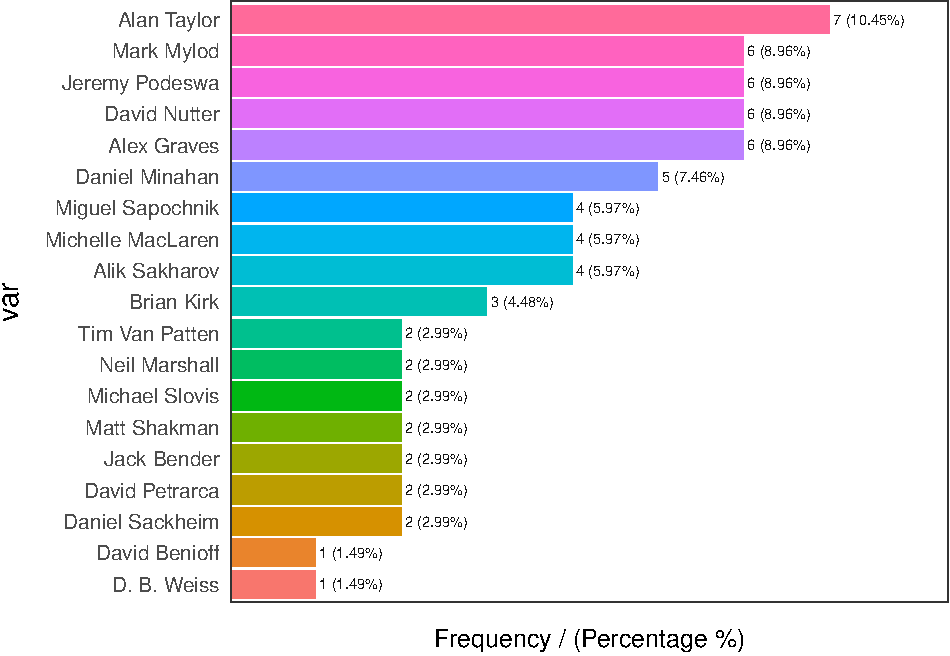
\includegraphics{FinalProject_files/figure-latex/unnamed-chunk-10-1.pdf}

\begin{Shaded}
\begin{Highlighting}[]
\NormalTok{Director <-}\StringTok{ }\KeywordTok{freq}\NormalTok{(gameofthrones}\OperatorTok{$}\NormalTok{Director)}
\end{Highlighting}
\end{Shaded}

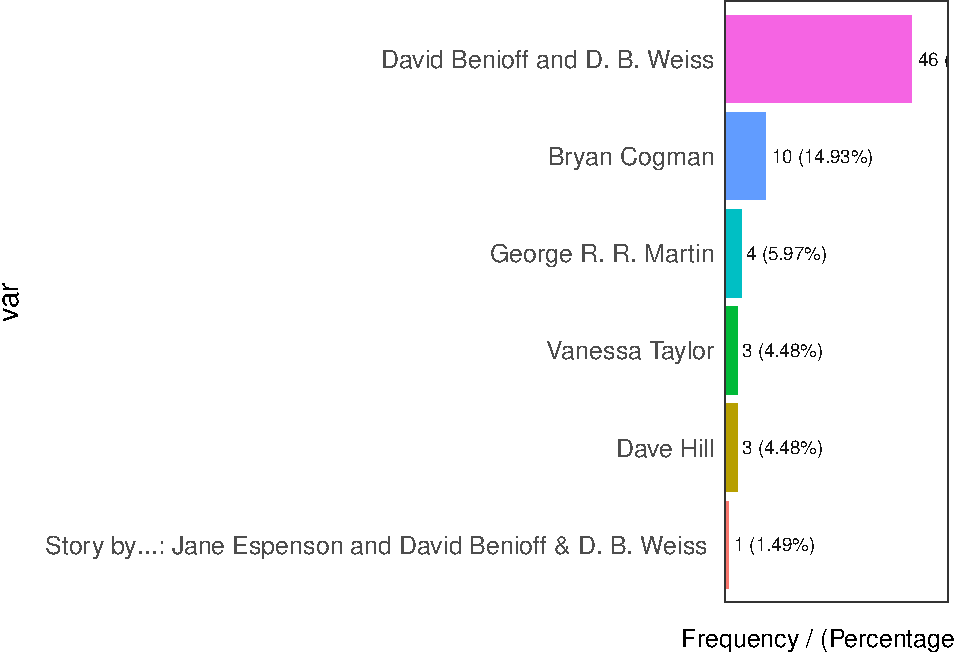
\includegraphics{FinalProject_files/figure-latex/unnamed-chunk-11-1.pdf}

\#\#```\{r\} got\_data\(Writer ab<-got_data\)Writer{[}1{]} \textless{}-
``xyz'' ab

\begin{Shaded}
\begin{Highlighting}[]
\NormalTok{Writer <-}\StringTok{ }\KeywordTok{freq}\NormalTok{(gameofthrones}\OperatorTok{$}\NormalTok{Writer)}
\end{Highlighting}
\end{Shaded}

\begin{verbatim}
## Warning in grid.Call(C_textBounds, as.graphicsAnnot(x$label), x$x, x$y, :
## conversion failure on 'Story by : Jane Espenson and David Benioff & D. B.
## Weiss ' in 'mbcsToSbcs': dot substituted for <e2>
\end{verbatim}

\begin{verbatim}
## Warning in grid.Call(C_textBounds, as.graphicsAnnot(x$label), x$x, x$y, :
## conversion failure on 'Story by : Jane Espenson and David Benioff & D. B.
## Weiss ' in 'mbcsToSbcs': dot substituted for <80>
\end{verbatim}

\begin{verbatim}
## Warning in grid.Call(C_textBounds, as.graphicsAnnot(x$label), x$x, x$y, :
## conversion failure on 'Story by : Jane Espenson and David Benioff & D. B.
## Weiss ' in 'mbcsToSbcs': dot substituted for <8a>
\end{verbatim}

\begin{verbatim}
## Warning in grid.Call(C_textBounds, as.graphicsAnnot(x$label), x$x, x$y, :
## conversion failure on 'Story by : Jane Espenson and David Benioff & D. B.
## Weiss ' in 'mbcsToSbcs': dot substituted for <e2>
\end{verbatim}

\begin{verbatim}
## Warning in grid.Call(C_textBounds, as.graphicsAnnot(x$label), x$x, x$y, :
## conversion failure on 'Story by : Jane Espenson and David Benioff & D. B.
## Weiss ' in 'mbcsToSbcs': dot substituted for <80>
\end{verbatim}

\begin{verbatim}
## Warning in grid.Call(C_textBounds, as.graphicsAnnot(x$label), x$x, x$y, :
## conversion failure on 'Story by : Jane Espenson and David Benioff & D. B.
## Weiss ' in 'mbcsToSbcs': dot substituted for <8a>
\end{verbatim}

\begin{verbatim}
## Warning in grid.Call(C_textBounds, as.graphicsAnnot(x$label), x$x, x$y, :
## conversion failure on 'Story by : Jane Espenson and David Benioff & D. B.
## Weiss ' in 'mbcsToSbcs': dot substituted for <e2>
\end{verbatim}

\begin{verbatim}
## Warning in grid.Call(C_textBounds, as.graphicsAnnot(x$label), x$x, x$y, :
## conversion failure on 'Story by : Jane Espenson and David Benioff & D. B.
## Weiss ' in 'mbcsToSbcs': dot substituted for <80>
\end{verbatim}

\begin{verbatim}
## Warning in grid.Call(C_textBounds, as.graphicsAnnot(x$label), x$x, x$y, :
## conversion failure on 'Story by : Jane Espenson and David Benioff & D. B.
## Weiss ' in 'mbcsToSbcs': dot substituted for <8a>
\end{verbatim}

\begin{verbatim}
## Warning in grid.Call(C_textBounds, as.graphicsAnnot(x$label), x$x, x$y, :
## conversion failure on 'Story by : Jane Espenson and David Benioff & D. B.
## Weiss ' in 'mbcsToSbcs': dot substituted for <e2>
\end{verbatim}

\begin{verbatim}
## Warning in grid.Call(C_textBounds, as.graphicsAnnot(x$label), x$x, x$y, :
## conversion failure on 'Story by : Jane Espenson and David Benioff & D. B.
## Weiss ' in 'mbcsToSbcs': dot substituted for <80>
\end{verbatim}

\begin{verbatim}
## Warning in grid.Call(C_textBounds, as.graphicsAnnot(x$label), x$x, x$y, :
## conversion failure on 'Story by : Jane Espenson and David Benioff & D. B.
## Weiss ' in 'mbcsToSbcs': dot substituted for <8a>
\end{verbatim}

\begin{verbatim}
## Warning in grid.Call(C_textBounds, as.graphicsAnnot(x$label), x$x, x$y, :
## conversion failure on 'Story by : Jane Espenson and David Benioff & D. B.
## Weiss ' in 'mbcsToSbcs': dot substituted for <e2>
\end{verbatim}

\begin{verbatim}
## Warning in grid.Call(C_textBounds, as.graphicsAnnot(x$label), x$x, x$y, :
## conversion failure on 'Story by : Jane Espenson and David Benioff & D. B.
## Weiss ' in 'mbcsToSbcs': dot substituted for <80>
\end{verbatim}

\begin{verbatim}
## Warning in grid.Call(C_textBounds, as.graphicsAnnot(x$label), x$x, x$y, :
## conversion failure on 'Story by : Jane Espenson and David Benioff & D. B.
## Weiss ' in 'mbcsToSbcs': dot substituted for <8a>
\end{verbatim}

\begin{verbatim}
## Warning in grid.Call(C_textBounds, as.graphicsAnnot(x$label), x$x, x$y, :
## conversion failure on 'Story by : Jane Espenson and David Benioff & D. B.
## Weiss ' in 'mbcsToSbcs': dot substituted for <e2>
\end{verbatim}

\begin{verbatim}
## Warning in grid.Call(C_textBounds, as.graphicsAnnot(x$label), x$x, x$y, :
## conversion failure on 'Story by : Jane Espenson and David Benioff & D. B.
## Weiss ' in 'mbcsToSbcs': dot substituted for <80>
\end{verbatim}

\begin{verbatim}
## Warning in grid.Call(C_textBounds, as.graphicsAnnot(x$label), x$x, x$y, :
## conversion failure on 'Story by : Jane Espenson and David Benioff & D. B.
## Weiss ' in 'mbcsToSbcs': dot substituted for <8a>
\end{verbatim}

\begin{verbatim}
## Warning in grid.Call(C_textBounds, as.graphicsAnnot(x$label), x$x, x$y, :
## conversion failure on 'Story by : Jane Espenson and David Benioff & D. B.
## Weiss ' in 'mbcsToSbcs': dot substituted for <e2>
\end{verbatim}

\begin{verbatim}
## Warning in grid.Call(C_textBounds, as.graphicsAnnot(x$label), x$x, x$y, :
## conversion failure on 'Story by : Jane Espenson and David Benioff & D. B.
## Weiss ' in 'mbcsToSbcs': dot substituted for <80>
\end{verbatim}

\begin{verbatim}
## Warning in grid.Call(C_textBounds, as.graphicsAnnot(x$label), x$x, x$y, :
## conversion failure on 'Story by : Jane Espenson and David Benioff & D. B.
## Weiss ' in 'mbcsToSbcs': dot substituted for <8a>
\end{verbatim}

\begin{verbatim}
## Warning in grid.Call(C_textBounds, as.graphicsAnnot(x$label), x$x, x$y, :
## conversion failure on 'Story by : Jane Espenson and David Benioff & D. B.
## Weiss ' in 'mbcsToSbcs': dot substituted for <e2>
\end{verbatim}

\begin{verbatim}
## Warning in grid.Call(C_textBounds, as.graphicsAnnot(x$label), x$x, x$y, :
## conversion failure on 'Story by : Jane Espenson and David Benioff & D. B.
## Weiss ' in 'mbcsToSbcs': dot substituted for <80>
\end{verbatim}

\begin{verbatim}
## Warning in grid.Call(C_textBounds, as.graphicsAnnot(x$label), x$x, x$y, :
## conversion failure on 'Story by : Jane Espenson and David Benioff & D. B.
## Weiss ' in 'mbcsToSbcs': dot substituted for <8a>
\end{verbatim}

\begin{verbatim}
## Warning in grid.Call(C_textBounds, as.graphicsAnnot(x$label), x$x, x$y, :
## conversion failure on 'Story by : Jane Espenson and David Benioff & D. B.
## Weiss ' in 'mbcsToSbcs': dot substituted for <e2>
\end{verbatim}

\begin{verbatim}
## Warning in grid.Call(C_textBounds, as.graphicsAnnot(x$label), x$x, x$y, :
## conversion failure on 'Story by : Jane Espenson and David Benioff & D. B.
## Weiss ' in 'mbcsToSbcs': dot substituted for <80>
\end{verbatim}

\begin{verbatim}
## Warning in grid.Call(C_textBounds, as.graphicsAnnot(x$label), x$x, x$y, :
## conversion failure on 'Story by : Jane Espenson and David Benioff & D. B.
## Weiss ' in 'mbcsToSbcs': dot substituted for <8a>
\end{verbatim}

\begin{verbatim}
## Warning in grid.Call(C_textBounds, as.graphicsAnnot(x$label), x$x, x$y, :
## conversion failure on 'Story by : Jane Espenson and David Benioff & D. B.
## Weiss ' in 'mbcsToSbcs': dot substituted for <e2>
\end{verbatim}

\begin{verbatim}
## Warning in grid.Call(C_textBounds, as.graphicsAnnot(x$label), x$x, x$y, :
## conversion failure on 'Story by : Jane Espenson and David Benioff & D. B.
## Weiss ' in 'mbcsToSbcs': dot substituted for <80>
\end{verbatim}

\begin{verbatim}
## Warning in grid.Call(C_textBounds, as.graphicsAnnot(x$label), x$x, x$y, :
## conversion failure on 'Story by : Jane Espenson and David Benioff & D. B.
## Weiss ' in 'mbcsToSbcs': dot substituted for <8a>
\end{verbatim}

\begin{verbatim}
## Warning in grid.Call(C_textBounds, as.graphicsAnnot(x$label), x$x, x$y, :
## conversion failure on 'Story by : Jane Espenson and David Benioff & D. B.
## Weiss ' in 'mbcsToSbcs': dot substituted for <e2>
\end{verbatim}

\begin{verbatim}
## Warning in grid.Call(C_textBounds, as.graphicsAnnot(x$label), x$x, x$y, :
## conversion failure on 'Story by : Jane Espenson and David Benioff & D. B.
## Weiss ' in 'mbcsToSbcs': dot substituted for <80>
\end{verbatim}

\begin{verbatim}
## Warning in grid.Call(C_textBounds, as.graphicsAnnot(x$label), x$x, x$y, :
## conversion failure on 'Story by : Jane Espenson and David Benioff & D. B.
## Weiss ' in 'mbcsToSbcs': dot substituted for <8a>
\end{verbatim}

\begin{verbatim}
## Warning in grid.Call(C_textBounds, as.graphicsAnnot(x$label), x$x, x$y, :
## conversion failure on 'Story by : Jane Espenson and David Benioff & D. B.
## Weiss ' in 'mbcsToSbcs': dot substituted for <e2>
\end{verbatim}

\begin{verbatim}
## Warning in grid.Call(C_textBounds, as.graphicsAnnot(x$label), x$x, x$y, :
## conversion failure on 'Story by : Jane Espenson and David Benioff & D. B.
## Weiss ' in 'mbcsToSbcs': dot substituted for <80>
\end{verbatim}

\begin{verbatim}
## Warning in grid.Call(C_textBounds, as.graphicsAnnot(x$label), x$x, x$y, :
## conversion failure on 'Story by : Jane Espenson and David Benioff & D. B.
## Weiss ' in 'mbcsToSbcs': dot substituted for <8a>
\end{verbatim}

\begin{verbatim}
## Warning in grid.Call(C_textBounds, as.graphicsAnnot(x$label), x$x, x$y, :
## conversion failure on 'Story by : Jane Espenson and David Benioff & D. B.
## Weiss ' in 'mbcsToSbcs': dot substituted for <e2>
\end{verbatim}

\begin{verbatim}
## Warning in grid.Call(C_textBounds, as.graphicsAnnot(x$label), x$x, x$y, :
## conversion failure on 'Story by : Jane Espenson and David Benioff & D. B.
## Weiss ' in 'mbcsToSbcs': dot substituted for <80>
\end{verbatim}

\begin{verbatim}
## Warning in grid.Call(C_textBounds, as.graphicsAnnot(x$label), x$x, x$y, :
## conversion failure on 'Story by : Jane Espenson and David Benioff & D. B.
## Weiss ' in 'mbcsToSbcs': dot substituted for <8a>
\end{verbatim}

\begin{verbatim}
## Warning in grid.Call(C_textBounds, as.graphicsAnnot(x$label), x$x, x$y, :
## conversion failure on 'Story by : Jane Espenson and David Benioff & D. B.
## Weiss ' in 'mbcsToSbcs': dot substituted for <e2>
\end{verbatim}

\begin{verbatim}
## Warning in grid.Call(C_textBounds, as.graphicsAnnot(x$label), x$x, x$y, :
## conversion failure on 'Story by : Jane Espenson and David Benioff & D. B.
## Weiss ' in 'mbcsToSbcs': dot substituted for <80>
\end{verbatim}

\begin{verbatim}
## Warning in grid.Call(C_textBounds, as.graphicsAnnot(x$label), x$x, x$y, :
## conversion failure on 'Story by : Jane Espenson and David Benioff & D. B.
## Weiss ' in 'mbcsToSbcs': dot substituted for <8a>
\end{verbatim}

\begin{verbatim}
## Warning in grid.Call(C_textBounds, as.graphicsAnnot(x$label), x$x, x$y, :
## conversion failure on 'Story by : Jane Espenson and David Benioff & D. B.
## Weiss ' in 'mbcsToSbcs': dot substituted for <e2>
\end{verbatim}

\begin{verbatim}
## Warning in grid.Call(C_textBounds, as.graphicsAnnot(x$label), x$x, x$y, :
## conversion failure on 'Story by : Jane Espenson and David Benioff & D. B.
## Weiss ' in 'mbcsToSbcs': dot substituted for <80>
\end{verbatim}

\begin{verbatim}
## Warning in grid.Call(C_textBounds, as.graphicsAnnot(x$label), x$x, x$y, :
## conversion failure on 'Story by : Jane Espenson and David Benioff & D. B.
## Weiss ' in 'mbcsToSbcs': dot substituted for <8a>
\end{verbatim}

\begin{verbatim}
## Warning in grid.Call.graphics(C_text, as.graphicsAnnot(x$label), x$x, x$y, :
## conversion failure on 'Story by : Jane Espenson and David Benioff & D. B.
## Weiss ' in 'mbcsToSbcs': dot substituted for <e2>
\end{verbatim}

\begin{verbatim}
## Warning in grid.Call.graphics(C_text, as.graphicsAnnot(x$label), x$x, x$y, :
## conversion failure on 'Story by : Jane Espenson and David Benioff & D. B.
## Weiss ' in 'mbcsToSbcs': dot substituted for <80>
\end{verbatim}

\begin{verbatim}
## Warning in grid.Call.graphics(C_text, as.graphicsAnnot(x$label), x$x, x$y, :
## conversion failure on 'Story by : Jane Espenson and David Benioff & D. B.
## Weiss ' in 'mbcsToSbcs': dot substituted for <8a>
\end{verbatim}

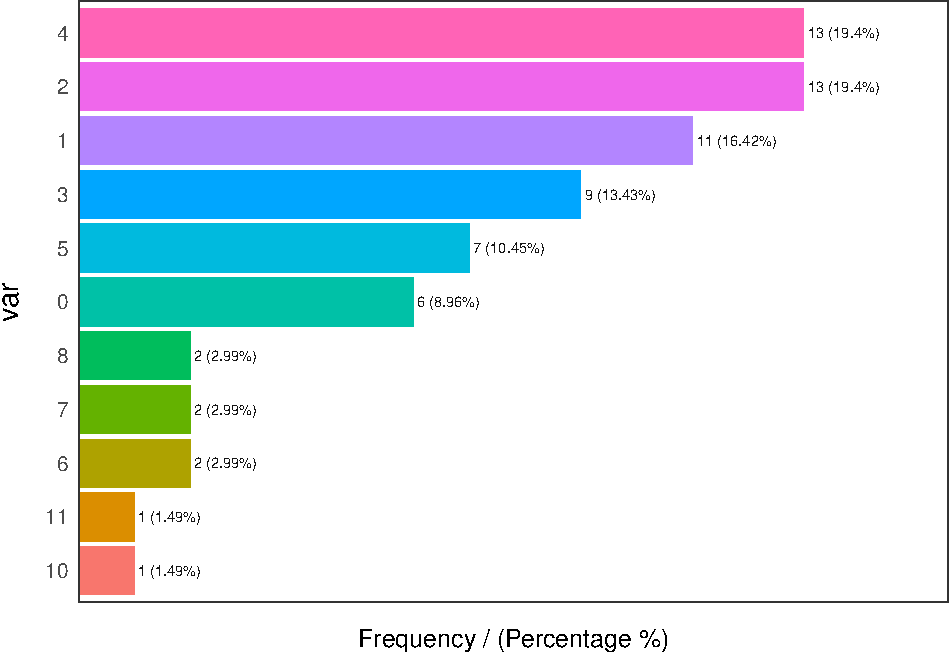
\includegraphics{FinalProject_files/figure-latex/unnamed-chunk-12-1.pdf}

\begin{Shaded}
\begin{Highlighting}[]
\NormalTok{NotableDeathCount <-}\StringTok{ }\KeywordTok{freq}\NormalTok{(gameofthrones}\OperatorTok{$}\NormalTok{Notable.Death.Count)}
\end{Highlighting}
\end{Shaded}

\includegraphics{FinalProject_files/figure-latex/unnamed-chunk-13-1.pdf}

\hypertarget{one-sample-test}{%
\subsection{One sample test}\label{one-sample-test}}

\begin{Shaded}
\begin{Highlighting}[]
\NormalTok{x_bar <-}\StringTok{ }\KeywordTok{mean}\NormalTok{(gameofthrones}\OperatorTok{$}\NormalTok{Imdb.Rating)}
\CommentTok{# null hypothesized population mean}
\NormalTok{mu_}\DecValTok{0}\NormalTok{ <-}\StringTok{ }\DecValTok{10}
\CommentTok{# sample st. dev}
\NormalTok{s <-}\StringTok{ }\KeywordTok{sd}\NormalTok{(gameofthrones}\OperatorTok{$}\NormalTok{Imdb.Rating)}
\CommentTok{# sample size}
\NormalTok{n <-}\StringTok{ }\KeywordTok{length}\NormalTok{(gameofthrones}\OperatorTok{$}\NormalTok{Imdb.Rating)}
\CommentTok{# t-test test statistic}
\NormalTok{t <-}\StringTok{ }\NormalTok{(x_bar }\OperatorTok{-}\StringTok{ }\NormalTok{mu_}\DecValTok{0}\NormalTok{)}\OperatorTok{/}\NormalTok{(s}\OperatorTok{/}\KeywordTok{sqrt}\NormalTok{(n))}
\CommentTok{# two-sided p-value so multiply by 2}
\NormalTok{two_sided_t_pval <-}\StringTok{ }\KeywordTok{pt}\NormalTok{(}\DataTypeTok{q =}\NormalTok{ t, }\DataTypeTok{df =}\NormalTok{ n}\DecValTok{-1}\NormalTok{)}\OperatorTok{*}\DecValTok{2}
\NormalTok{two_sided_t_pval}
\end{Highlighting}
\end{Shaded}

\begin{verbatim}
## [1] 4.456761e-26
\end{verbatim}

\hypertarget{wrong-graph-but-needed}{%
\subsection{wrong graph but needed}\label{wrong-graph-but-needed}}

\begin{Shaded}
\begin{Highlighting}[]
\CommentTok{# plot a t-distribution with n-1 df}
\KeywordTok{plot}\NormalTok{(}\KeywordTok{seq}\NormalTok{(}\OperatorTok{-}\DecValTok{20}\NormalTok{, }\DecValTok{20}\NormalTok{, }\FloatTok{.01}\NormalTok{), }\KeywordTok{dt}\NormalTok{(}\KeywordTok{seq}\NormalTok{(}\OperatorTok{-}\DecValTok{20}\NormalTok{, }\DecValTok{20}\NormalTok{, }\FloatTok{.01}\NormalTok{), n}\DecValTok{-1}\NormalTok{), }\DataTypeTok{type=}\StringTok{"l"}\NormalTok{)}
\CommentTok{# add the lines for my test statistic}
\KeywordTok{abline}\NormalTok{(}\DataTypeTok{v=}\KeywordTok{c}\NormalTok{(t, }\OperatorTok{-}\NormalTok{t))}
\KeywordTok{text}\NormalTok{(t,.}\DecValTok{025}\NormalTok{,}\StringTok{"t=-17.389962"}\NormalTok{,}\DataTypeTok{srt=}\FloatTok{0.2}\NormalTok{,}\DataTypeTok{pos=}\DecValTok{4}\NormalTok{)}
\KeywordTok{text}\NormalTok{(}\OperatorTok{-}\NormalTok{t,.}\DecValTok{025}\NormalTok{,}\StringTok{"t=17.389962"}\NormalTok{,}\DataTypeTok{srt=}\FloatTok{0.2}\NormalTok{,}\DataTypeTok{pos=}\DecValTok{2}\NormalTok{)}
\CommentTok{# add the lines for the t-critical value associated with alpha=0.05 and n-1 degrees of freedom}
\CommentTok{# two-sided so in each tail we should have 2.5% of the probability}
\KeywordTok{abline}\NormalTok{(}\DataTypeTok{v=}\KeywordTok{c}\NormalTok{(}\KeywordTok{qt}\NormalTok{(}\FloatTok{0.025}\NormalTok{, n}\DecValTok{-1}\NormalTok{), }\KeywordTok{qt}\NormalTok{(}\FloatTok{0.975}\NormalTok{, n}\DecValTok{-1}\NormalTok{)))}
\KeywordTok{text}\NormalTok{(}\KeywordTok{qt}\NormalTok{(}\FloatTok{0.025}\NormalTok{, n}\DecValTok{-1}\NormalTok{), }\FloatTok{0.07}\NormalTok{, }\StringTok{"t=-2.042272"}\NormalTok{,}\DataTypeTok{srt=}\FloatTok{0.2}\NormalTok{,}\DataTypeTok{pos=}\DecValTok{2}\NormalTok{)}
\KeywordTok{text}\NormalTok{(}\KeywordTok{qt}\NormalTok{(}\FloatTok{0.975}\NormalTok{, n}\DecValTok{-1}\NormalTok{), }\FloatTok{0.07}\NormalTok{, }\StringTok{"t=2.042272"}\NormalTok{,}\DataTypeTok{srt=}\FloatTok{0.2}\NormalTok{,}\DataTypeTok{pos=}\DecValTok{4}\NormalTok{)}
\end{Highlighting}
\end{Shaded}

\includegraphics{FinalProject_files/figure-latex/unnamed-chunk-15-1.pdf}

\hypertarget{confidence-interval}{%
\subsection{Confidence Interval}\label{confidence-interval}}

\begin{Shaded}
\begin{Highlighting}[]
\CommentTok{# lower bound}
\NormalTok{x_bar}\OperatorTok{+}\NormalTok{(}\KeywordTok{qt}\NormalTok{(}\FloatTok{0.025}\NormalTok{, n}\DecValTok{-1}\NormalTok{)}\OperatorTok{*}\NormalTok{(s}\OperatorTok{/}\KeywordTok{sqrt}\NormalTok{(n))) }
\end{Highlighting}
\end{Shaded}

\begin{verbatim}
## [1] 9.008845
\end{verbatim}

\begin{Shaded}
\begin{Highlighting}[]
\CommentTok{# alternately you can use x_bar-(qt(0.975, n-1)*(s/sqrt(n)))}
\CommentTok{# upper bound}
\NormalTok{x_bar}\OperatorTok{+}\NormalTok{(}\KeywordTok{qt}\NormalTok{(}\FloatTok{0.975}\NormalTok{, n}\DecValTok{-1}\NormalTok{)}\OperatorTok{*}\NormalTok{(s}\OperatorTok{/}\KeywordTok{sqrt}\NormalTok{(n))) }
\end{Highlighting}
\end{Shaded}

\begin{verbatim}
## [1] 9.215036
\end{verbatim}

\begin{Shaded}
\begin{Highlighting}[]
\CommentTok{# alternately you can use x_bar-(qt(0.025, n-1)*(s/sqrt(n)))}
\end{Highlighting}
\end{Shaded}

\begin{Shaded}
\begin{Highlighting}[]
\KeywordTok{qqnorm}\NormalTok{(gameofthrones}\OperatorTok{$}\NormalTok{Imdb.Rating)}
\end{Highlighting}
\end{Shaded}

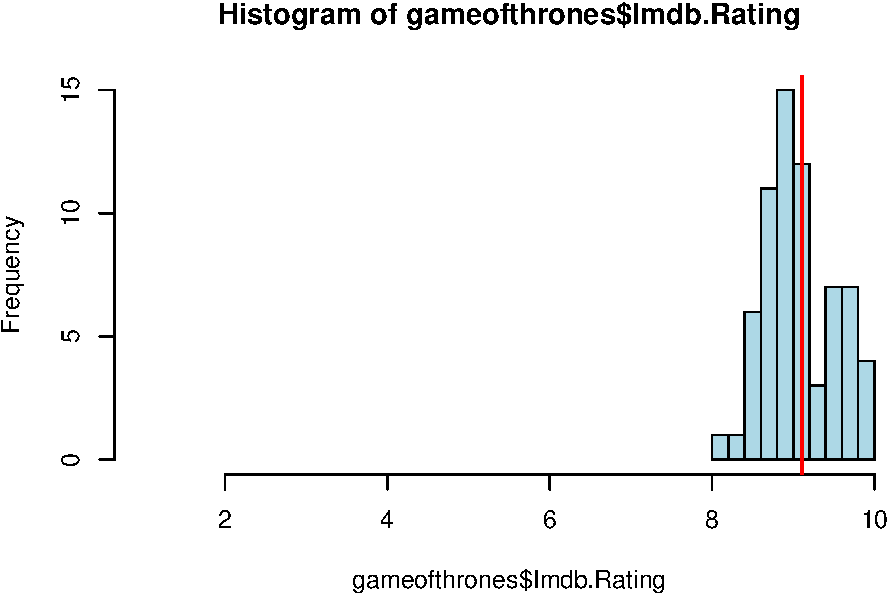
\includegraphics{FinalProject_files/figure-latex/unnamed-chunk-17-1.pdf}

\#\#on
\#\#\texttt{\{r\}\ ggplot(got\_data)\ +\ \ \ geom\_bar(aes(x\ =\ season,\ fill\ =\ season))\ +\ \ \ labs(x\ =\ \textquotesingle{}\textquotesingle{},\ y\ =\ \textquotesingle{}\textquotesingle{},\ title\ =\ \textquotesingle{}Number\textquotesingle{})\ +\ \ \ guides(fill\ =\ FALSE)\ \#\#}

\#\#\texttt{\{r,\ warning=FALSE,\ message=FALSE\}\ \#\#hist(data\$Season)\ \#\#}

\#\#```\{r\} \# Pie Chart with Percentages

pct \textless{}- (slices/sum()*100) lbls \textless{}- paste(lbls, pct)
\# add percents to labels lbls \textless{}- paste(lbls,``\%'',sep="``)
\# ad \% to labels pie(slices,labels = lbls, col=rainbow(length(lbls)),
main=''Pie Chart of Countries") \#\#```

\begin{Shaded}
\begin{Highlighting}[]
\KeywordTok{hist}\NormalTok{(gameofthrones}\OperatorTok{$}\NormalTok{Imdb.Rating, }
 \DataTypeTok{xlim =} \KeywordTok{c}\NormalTok{(}\DecValTok{1}\NormalTok{, }\DecValTok{10}\NormalTok{),}\CommentTok{##breaks = 5}
 \DataTypeTok{col =} \StringTok{"light blue"}\NormalTok{)}

\KeywordTok{abline}\NormalTok{(}\DataTypeTok{v =} \KeywordTok{mean}\NormalTok{(gameofthrones}\OperatorTok{$}\NormalTok{Imdb.Rating, }\DataTypeTok{na.rm =}\NormalTok{ T),}
            \DataTypeTok{col =} \StringTok{"red"}\NormalTok{,}
            \DataTypeTok{lwd =} \DecValTok{2}\NormalTok{)}
\end{Highlighting}
\end{Shaded}

\includegraphics{FinalProject_files/figure-latex/unnamed-chunk-18-1.pdf}

\begin{Shaded}
\begin{Highlighting}[]
\NormalTok{Avg <-}\StringTok{ }\KeywordTok{mean}\NormalTok{(gameofthrones}\OperatorTok{$}\NormalTok{Imdb.Rating)}
\KeywordTok{cat}\NormalTok{(}\StringTok{"Average No of rating: "}\NormalTok{ , Avg)}
\end{Highlighting}
\end{Shaded}

\begin{verbatim}
## Average No of rating:  9.11194
\end{verbatim}

\hypertarget{one-sample-proportion}{%
\subsection{One sample proportion}\label{one-sample-proportion}}

Which season is most popular? Let's find all the seasons which have
rating less than 9 and seasons which has maximum number of 9s

\begin{Shaded}
\begin{Highlighting}[]
\NormalTok{MostPopular <-}\StringTok{ }\NormalTok{gameofthrones }\OperatorTok\StringTok{ }\KeywordTok{select}\NormalTok{(}\DecValTok{1}\NormalTok{, }\DecValTok{12}\NormalTok{)}
\CommentTok{##MostPopular}
\NormalTok{MostPopular}\OperatorTok{$}\NormalTok{Imdb.Rating =}\StringTok{ }\KeywordTok{as.integer}\NormalTok{(MostPopular}\OperatorTok{$}\NormalTok{Imdb.Rating)}

\NormalTok{MostPopular}\OperatorTok{$}\NormalTok{Imdb.Rating[MostPopular}\OperatorTok{$}\NormalTok{Imdb.Rating }\OperatorTok{>=}\StringTok{ }\DecValTok{9}\NormalTok{] =}\StringTok{ 'Popular'}
\NormalTok{MostPopular}\OperatorTok{$}\NormalTok{Imdb.Rating[MostPopular}\OperatorTok{$}\NormalTok{Imdb.Rating }\OperatorTok{<}\StringTok{ }\DecValTok{9}\NormalTok{] =}\StringTok{ 'Not Popular'}
\NormalTok{MostPopular}
\end{Highlighting}
\end{Shaded}

\begin{verbatim}
##    Season Imdb.Rating
## 1       1     Popular
## 2       1 Not Popular
## 3       1 Not Popular
## 4       1 Not Popular
## 5       1     Popular
## 6       1     Popular
## 7       1     Popular
## 8       1     Popular
## 9       1     Popular
## 10      1     Popular
## 11      2 Not Popular
## 12      2 Not Popular
## 13      2 Not Popular
## 14      2 Not Popular
## 15      2 Not Popular
## 16      2     Popular
## 17      2     Popular
## 18      2 Not Popular
## 19      2     Popular
## 20      2     Popular
## 21      3 Not Popular
## 22      3 Not Popular
## 23      3 Not Popular
## 24      3     Popular
## 25      3     Popular
## 26      3 Not Popular
## 27      3 Not Popular
## 28      3     Popular
## 29      3     Popular
## 30      3     Popular
## 31      4     Popular
## 32      4     Popular
## 33      4 Not Popular
## 34      4 Not Popular
## 35      4 Not Popular
## 36      4     Popular
## 37      4     Popular
## 38      4     Popular
## 39      4     Popular
## 40      4     Popular
## 41      5 Not Popular
## 42      5 Not Popular
## 43      5 Not Popular
## 44      5 Not Popular
## 45      5 Not Popular
## 46      5 Not Popular
## 47      5     Popular
## 48      5     Popular
## 49      5     Popular
## 50      5     Popular
## 51      6 Not Popular
## 52      6     Popular
## 53      6 Not Popular
## 54      6     Popular
## 55      6     Popular
## 56      6 Not Popular
## 57      6 Not Popular
## 58      6 Not Popular
## 59      6     Popular
## 60      6     Popular
## 61      7 Not Popular
## 62      7     Popular
## 63      7     Popular
## 64      7     Popular
## 65      7     Popular
## 66      7     Popular
## 67      7     Popular
\end{verbatim}

\begin{Shaded}
\begin{Highlighting}[]
\NormalTok{x =}\StringTok{ }\KeywordTok{barplot}\NormalTok{(}\KeywordTok{prop.table}\NormalTok{(}\KeywordTok{table}\NormalTok{(MostPopular}\OperatorTok{$}\NormalTok{Imdb.Rating)), }\DataTypeTok{main =} \StringTok{'Barplot of episode popularity'}\NormalTok{, }\DataTypeTok{xlab =} \StringTok{'Imdb rating for season-wise '}\NormalTok{, }\DataTypeTok{ylab =} \StringTok{'Percentage of People'}\NormalTok{, }\DataTypeTok{ylim =} \KeywordTok{c}\NormalTok{(}\DecValTok{0}\NormalTok{,}\FloatTok{0.6}\NormalTok{))}

\KeywordTok{text}\NormalTok{(x, }\KeywordTok{prop.table}\NormalTok{(}\KeywordTok{table}\NormalTok{(MostPopular}\OperatorTok{$}\NormalTok{Imdb.Rating)), }\DataTypeTok{labels =} \KeywordTok{paste}\NormalTok{(}\KeywordTok{round}\NormalTok{(}\KeywordTok{prop.table}\NormalTok{(}\KeywordTok{table}\NormalTok{(MostPopular}\OperatorTok{$}\NormalTok{Imdb.Rating)), }\DataTypeTok{digits =} \DecValTok{4}\NormalTok{)}\OperatorTok{*}\DecValTok{100}\NormalTok{, }\StringTok{"%"}\NormalTok{) ,}\DataTypeTok{cex=}\DecValTok{1}\NormalTok{, }\DataTypeTok{col =} \StringTok{"blue"}\NormalTok{, }\DataTypeTok{pos =} \DecValTok{1}\NormalTok{) }
\end{Highlighting}
\end{Shaded}

\includegraphics{FinalProject_files/figure-latex/unnamed-chunk-21-1.pdf}

\end{document}
